\section{The A3-E Model}\label{sec:proposal}

\begin{figure}[tbp]
	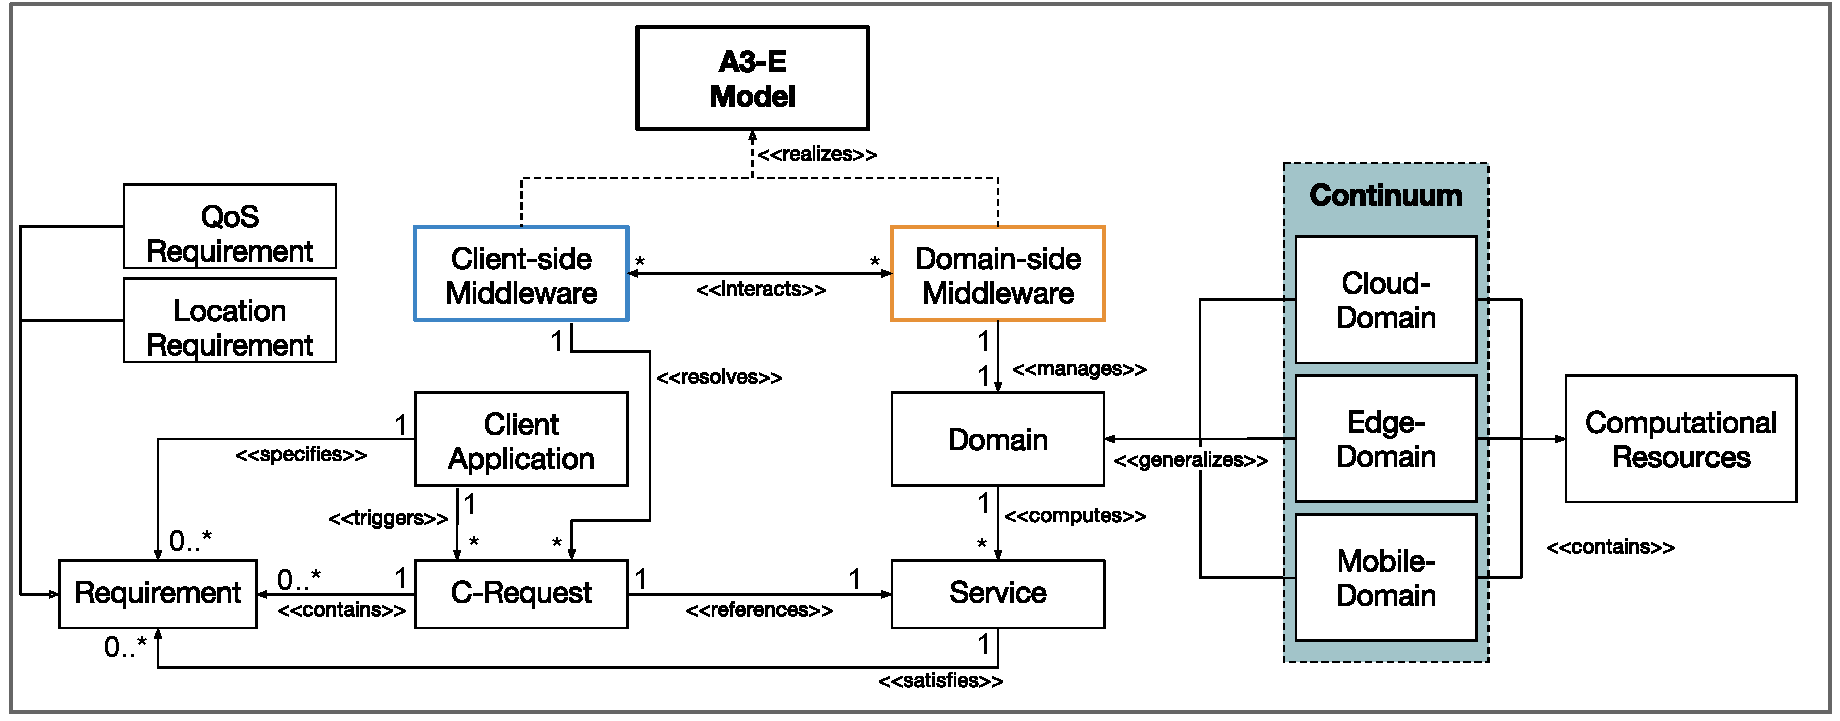
\includegraphics[width=1\textwidth]{figs/A3-E-model.pdf}
	\caption{The A3-E Model.}
	\label{fig:A3-E-model}
\end{figure}

The \textit{A3-E model}, depicted in Fig.~\ref{fig:A3-E-model}, defines the actors and mechanisms required to realize the computing continuum. It inherits its name from its four phases -- namely, \textit{(\textbf{A}wareness), (\textbf{A})cquisition, (\textbf{A})llocation, and (\textbf{E})ngagement}. Each phase addresses specific concerns in the interaction between client applications and the service providers in the continuum. The model is flexible with respect to which (and how) phases are actually employed, to address the intrinsic heterogeneity of the continuum. 

A3-E exploits the Serverless Architecture~\cite{baldini2017serverless} to guarantee that the heterogeneous service providers in the continuum are efficient, scalable and automatable~\cite{GarrigaMendonca2017,Hendrickson:2016}. 

Serverless is a cloud computing model in which business functionality is provided without pre-allocating computational resources. Instead, shared resources (e.g. containers) are used to provision and execute functions on demand, in only a few milliseconds. Particularly, A3-E embraces the Function-as-a-Service (FaaS) execution model~\cite{MateosFaaster17}, where functions are ephemeral (they may even last for only one invocation), stateless, and scaled as needed~\cite{Roberts:2016}. This approach allows one to write and deploy functions (code) without considering the server runtime environment, resource allocation, load balancing, or scalability; all these aspects are automatically handled by the provider --- hence the term serverless.

In the A3-E model, a \textit{service} is a set of artifacts that fulfill certain functionality and can be deployed to and accessed from a remote server. In particular, service artifacts can refer to: (i) the stateless function(s) exposed to the clients (e.g., a Java compiled class); (ii) static data (e.g., a trained neural network model); and (iii) other dependencies (e.g.,  software libraries). Moreover, these services are \textit{microservices}~\cite{lewis2014microservices}, as they are small, modular, communicate with lightweight mechanisms (often an HTTP RESTful API) and are independently deployable by fully automated machinery. 

A3-E microservices are provided by \textit{domain}s. A domain yields a common abstraction for the constituents of the continuum. Indeed, it hides the fact that they make use of heterogeneous \textit{computational resources} (e.g., server(s), virtual machine(s), container(s), memory, CPU, storage, etc.) and networking infrastructures (e.g., access points, radio access networks, etc.). Examples of A3-E domains are \textit{cloud-domains}, i.e., cloud-based FaaS platforms covering a specific geographical region (e.g., AWS Lambda\footnote{\url{https://aws.amazon.com/lambda}} in Europe); \textit{edge-domains}, representing local-edge and mobile-edge sites (e.g., servers within an office building or at cellular base stations); and \textit{mobile-domain}, representing a client device's own resources.


A3-E also defines \textit{client applications} as the software components responsible for sending \textit{C-requests} to the continuum. A C-request is an HTTP request with additional headers specifying requirements for the targeted microservice in the continuum. Two types of requirements are considered: \textit{QoS requirements}, that specifies QoS metrics (e.g., maximum latency, minimum availability, etc); and \textit{Location requirements}, that fixes the types of domain that may be used (e.g., mobile or edge, mobile only, cloud, etc). 

%TODO: who handles the client application request? A client-side middleware. Why its description was removed? The same question for the domain-side middleware. They are not just implementations, but part of the model. [Danilo]

%The figure has been placed here to avoid multiple diagrams in the same page [Danilo]

\begin{figure}[tbp]
	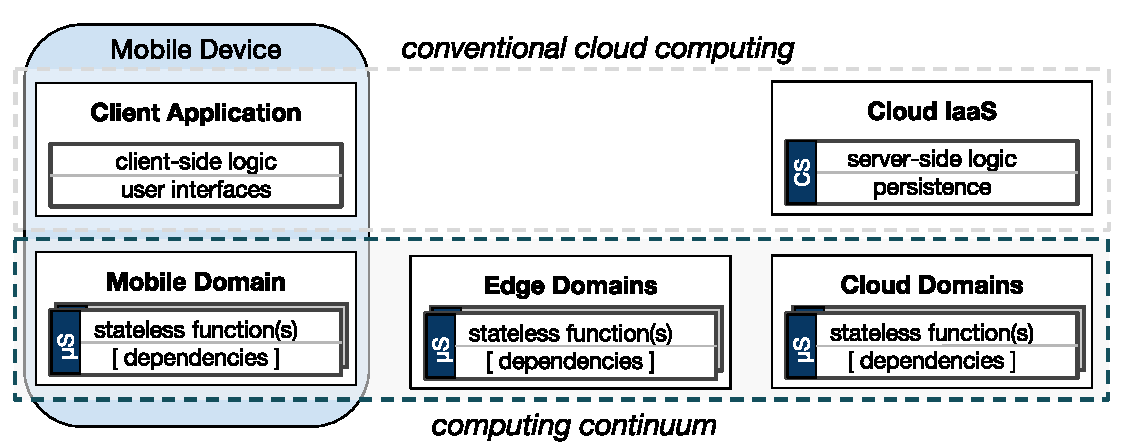
\includegraphics[width=0.9\textwidth]{figs/Continuum-arch}
	\caption{The high level architecture of a mobile application exploiting both the computing continuum -- by means of microservices ($\mu$S) provided by mobile, edge, and cloud domains -- and conventional cloud computing -- by means of cloud services (CS).}
	\label{fig:Continuum-arch}
\end{figure}

Figure~\ref{fig:Continuum-arch} illustrates the architecture of a \texttt{client application} --deployed to a mobile device-- that exploits both the continuum and conventional cloud infrastructure (IaaS). 

The client application comprises both \texttt{client-side logic} and \texttt{graphical user interfaces}. While the cloud infrastructure is used for \texttt{server-side logic} and for \texttt{persistence}, the continuum is used for stateless computation, provided by \texttt{stateless functions} that are exposed as \texttt{microservices}.

Although the continuum can hypothetically support any number of heterogeneous infrastructures, Figure~\ref{fig:Continuum-arch} focuses on three domains. The \texttt{Mobile Domain} is deployed to the client's mobile device, and provides local stateless computation. While enabling device-to-device collaboration through distributed mobile domains --i.e., by allowing a client to call a microservice deployed on another mobile device-- is surely interesting, for now we consider it part of our future work. The \texttt{Edge Domains} refer to Edge-based infrastructure that can be deployed to a local server (Local-Edge Domain) or to cellular stations (Mobile-Edge Domain). Finally, the \texttt{Cloud Domain} refers to a cloud-based solution such to AWS Lambda.

Considering our running example, the client-side mobile game application consists of controllers and user interfaces. The continuum provide the functionality for processing and updating the game state, which must be passed as parameter to a microservice in the continuum in conjunction with game events (e.g., user inputs). Finally, it also includes cloud services providing stateful server-side logic (e.g. authentication, business logic) and persistence (e.g., player scores). 

Also in our running example, the client-side AR application captures scenes from the glasses' camera and relies on the microservices in the continuum to extract features from objects in the scene (e.g., the user's desk, hands, crafting tools) based on a neural network trained model (composing the microservice dependencies) and an image processing library (available in the microservice runtime environment). Client-side logic is then responsible for updating the 3D virtual object state and render it into the scene displayed by the glasses. In this application, conventional cloud services are not required.


%\subsection*{Functions-as-a-Service (FaaS)}

%TODO compare bellow
%Aligned to our previous work~\cite{GarrigaMendonca2017}, A3-E addresses the efficiency required by edge domains by adhering to the FaaS execution model in which stateless functions can be allocated on demand without minimum pre-allocation of resources. The same model is employed by cloud-domains, which enables a uniform execution model among cloud and edge. In turn, mobile domains are exempt of implementing the allocation phase, as in this work we assume local services to be allocated along with the client application. 



%We consider conventional cloud services to be outside of the continuum because they can host virtually any type of application, apart from those that are continuum-compliant. 
%TODO let's discuss among us where is the best place to add this; here it must have already been said, probably in the explanation about serverless in the previous paragraph [Danilo]

% in which stateless functions can be allocated on demand without minimum pre-allocation of resources. 
%Such an architecture is already employed by multiple cloud providers\footnote{\url{https://blog.zhaw.ch/icclab/faas-function-hosting-services-and-their-technical-characteristics}}; its adoption by edge providers would have the following benefits: 1) \textit{scalability}, with the delegation of resource management; 2) \textit{efficiency}, with the provisioning of functions on demand without pre-allocation of computational resources; and 3) \textit{portability}, as functions are stateless and may be implemented in different languages, including those supported by mobile platforms. 

%The serverless architecture represents the latest step in the recent shift of enterprise application architectures to containers and microservices~\cite{baldini2017serverless}, which also allows the A3-E model to overcome the heterogeneity of the continuum by adhering to service-oriented principles. 

The four phases in A3-E, depicted in Figure~\ref{fig:A3-E-process}, support the self-management of microservice life-cycles. For each phase, A3-E  models the activities of both the \textit{domain} and of the \textit{client}. 

Next, we shall describe each of the four phases, starting from the most general one, i.e., the one that applies to all domains and clients, and moving towards the more specific ones. Keep in mind that in certain domains, one or more phases might not be employed.

%from the moment they become aware of each other to the point they may engage in client-server interactions

\begin{figure}[tbp]
	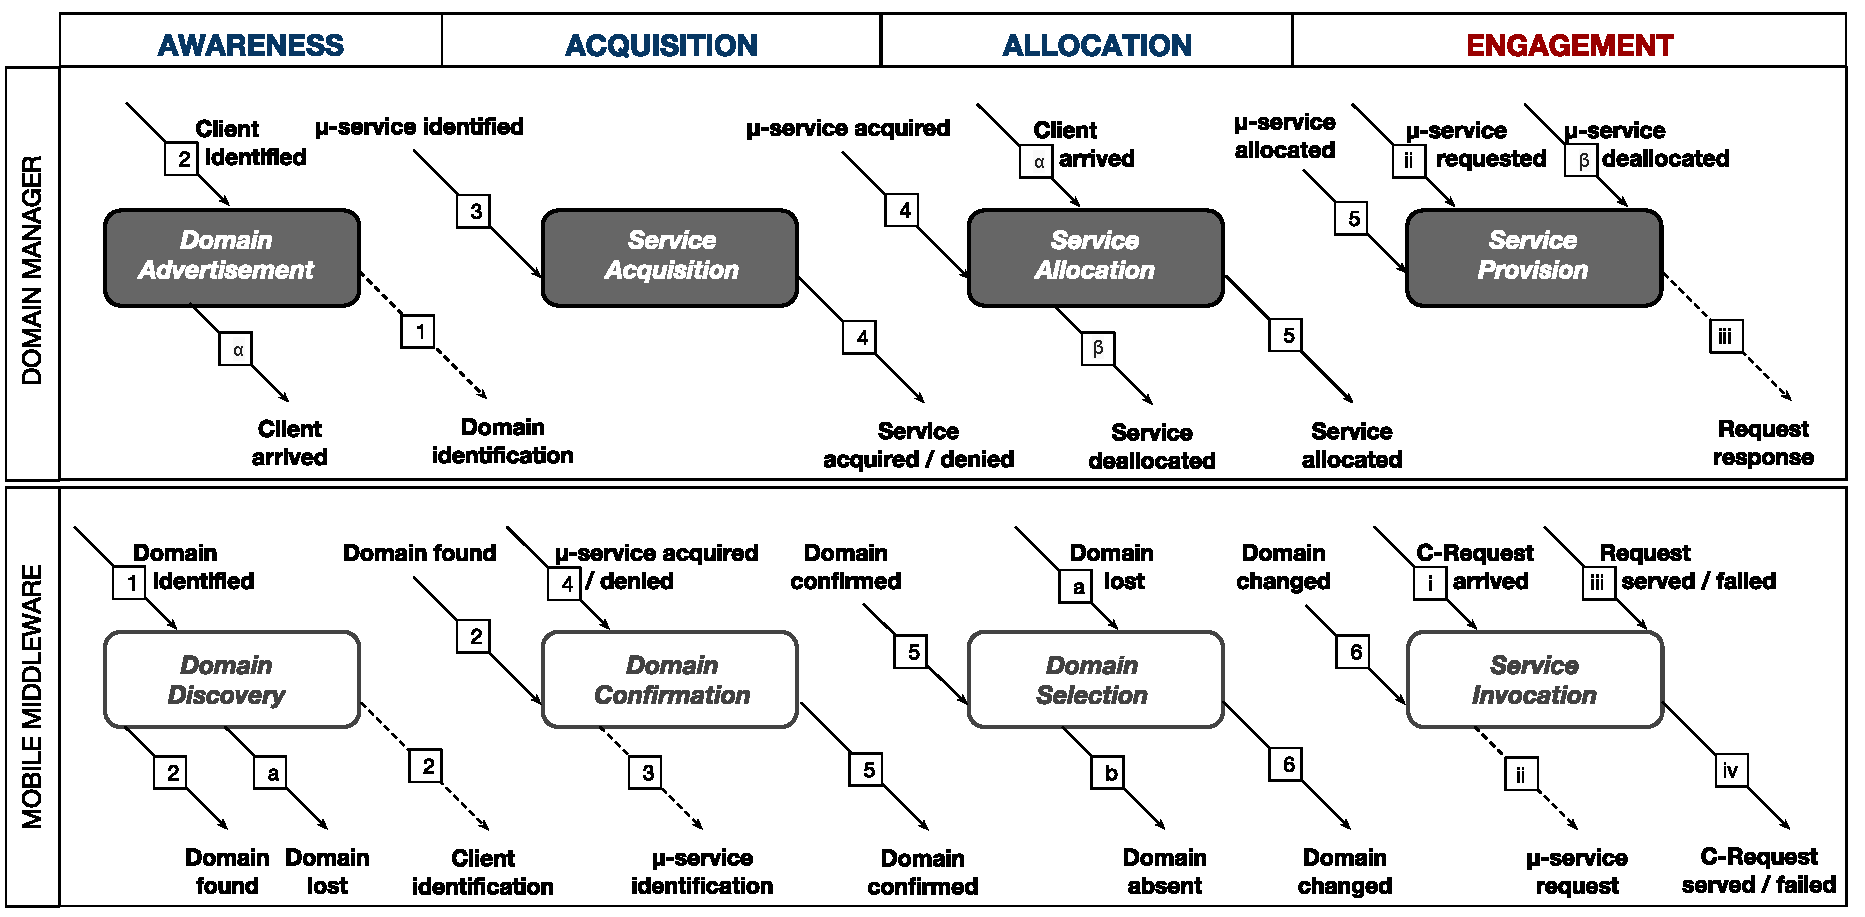
\includegraphics[width=0.95\textwidth]{figs/A3-E-process}
	\caption{The A3-E Process. Phases are delimited by vertical lines. The main activity of each phase is identified by the label within the phase; labels within parenthesis represent the states of a domain to a client (and vice-versa).}
	\label{fig:A3-E-process}
\end{figure}

%\subsection{A3-E Process: Phases}\label{sec:A3-E-process}

%Next, the four A3-E phases are further described and mapped to the requirements elicited in  Section~\ref{sec:requirements}. Later on, other possible instances of the A3-E model are correlated with scenarios of the compute continuum.

\subsection*{Engagement Phase}\label{sec:A3-E-engagement}

The \textit{engagement} phase models the last stage of interaction between a client application and a provider. Throughout this phase, clients engage with edge and cloud \textit{microservices} using a request/response protocol (e.g., RESTful microservices over HTTP). 

To enforce a common interface between clients and heterogeneous microservice providers in the continuum, mobile domains also expose microservices implemented with stateless functions. In fact, the FaaS execution model favors this architectural decision, as similar functions may be executed by a mobile domain's runtime (e.g., a Java runtime in an Android platform) or by FaaS platforms from different providers (e.g., a Java runtime provided by Apache OpenWhisk~\footnote{A well known open source serverless platform -- \url{http://openwhisk.incubator.apache.org/}} or AWS Lambda).

%In this phase the request has already been provisioned by one or more domains and the client-side middleware (CSM) has already selected a specific domain to make the request. 


%handled and parsed by the client-side middleware (CSM), and . 


%Also, one or more domains must have setup and allocated the requested service for execution and the CSM must have selected a specific domain among all providing the same service. Finally, client's request are sent, processed, received, and returned to the application.

%Current FaaS providers allow functions to be exposed as REST services. The same applies to open source platforms implementing the FaaS model. Finally, different approaches may be used to expose local computation as services in mobile platforms like Android and iOS.

%As an exception, computation provided by mobile devices can be accessed by means of local calls to functions executed by the mobile platform.

\subsection*{Allocation Phase}\label{sec:A3-E-allocation}

\begin{figure}[thbp]
	\centering
	\captionsetup[subfigure]{width=0.4\textwidth}	
	\null\hfill
	\subfloat[Microservices allocation control loop; domains must monitor the QoS of deployed microservices and adapt its allocation scheme to prevent SLA violation\label{fig:service-allocation-loop}]{ 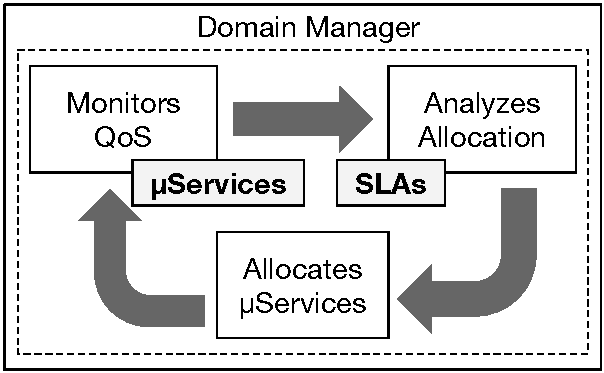
\includegraphics[width=0.4\textwidth]{figs/service-allocation-loop}}
	\captionsetup[subfigure]{width=0.4\textwidth}	
	\hfill
	\subfloat[Domain selection control loop; clients monitor microservices from available domains and select the one that best satisfies its requirements.\label{fig:domain-selection-loop}] {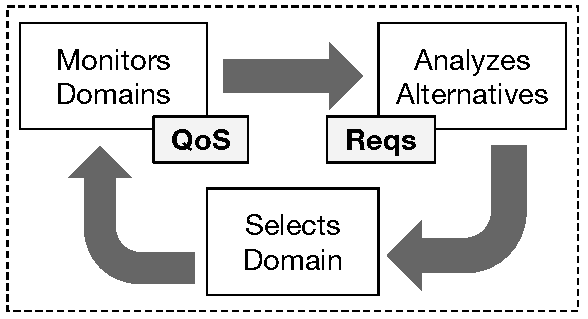
\includegraphics[width=0.4\textwidth]{figs/domain-selection-loop}}
	\hfill\null
	\caption{Self-management loops for domain-side microservices allocation and client-side microservice selection}\label{fig:allocation-loops}
\end{figure}

From the domain's perspective, the allocation phase models how the microservices are placed on the domain's resources, i.e., the intra-domain placement of microservices to its pool of servers, virtual machines, and containers. 

The scope of the domain-side allocation is limited by the domain's boundaries set by its provider. For instance, cloud domains allocate functions to containers in resourceful datacenters covering a large area. In turn, an edge domain may consist of a single server (e.g., covering an office) with a set of containers or distributed servers and containers covering an edge site (e.g., covering a whole building or a 5G base station).

%Traditionally, cloud domains employ automated scaling mechanisms in which virtual machines and container instances are (de)allocated on demand. More recently, cloud-based FaaS platforms (e.g., Amazon Lambda, Google Cloud Functions) extend these mechanisms to stateless functions. The later represent an extreme type of allocation in which no pre-allocation of resources is needed and functions are executed by a shared runtime platform. 


The domain-side middleware (DSM) exploits a self-management control loop~\cite{kephart2003vision} (see Figure~\ref{fig:service-allocation-loop}) in which the microservices are instantiated according to: (i) a monitored QoS (e.g., the availability of each microservice), (ii) a Service-Level Agreement (SLA), and (iii) the availability of the computational resources. 

%Once , the DSM informs the client whether the microservices can be considered ``acquired'' or not.

%For instance, in a centralized implementation, the DSM orchestrates the placement of functions to containers distributed along multiple servers.

While in cloud domains scalability is virtually unlimited, in finely distributed edge domains scalability needs to be prioritized to favor applications with more demanding requirements. For instance, edge providers could support two types of SLAs: one for critical applications requiring high availability, and another for non-critical applications that may cope with lower degrees of availability.  

%The first type could be achieved with the pre-allocation of resources to these services, whilst the latter could rely on the opportunistic allocation of services upon demand and availability of resources. 
In the scenario introduced in Section~\ref{sec:example}, the AV application should have a higher priority with respect to non-critical applications such as AR applications for turists~\cite{GarrigaMendonca2017}. In this case the edge microservices might become unavailable to the AR applications, for example during rush hour. In that case the AR and other low-priority applications would have to rely on microservices being run in the mobile domain, or in a cloud domain.

%The specific algorithms for the placement of services among the domain's resources that should be employed at the analysis phase are out of the scope of this paper. Nonetheless, recent works~\cite{} have addressed this challenge in the context of a continuum formed by edge and cloud datacenters. 

From the client's perspective, the allocation phase models the selection of the domain alternative that best satisfies the client's needs. Once again a self-management control loop is exploited (see Fig.~\ref{fig:domain-selection-loop}). 

The adopted microservice architecture based on stateless functions enables the selection of distinct microservices provided by different available domains. In each instance of its control loop, the CSM checks the QoS levels of a specific microservice from available domains. It then analyses and decides for the alternative best satisfying the application requirements.

%, i.e., it models the computation placement along the client's perception of the continuum. 
%This decision should consider a list of available domains providing services requested by the client application with accompanying QoS attributes. Accordingly, whereas the domains should take care of intra-domain allocation through service placement, the clients are responsible for the inter-domain allocation through service selection.

%Analogously to the domain-side, the CSM manages allocation with a self-management loop , this time by checking QoS levels of services from each available domain and deciding for the alternative that best satisfies the client's requirements. 

%This sub-process is the main client-side activity required for the realization of the continuum, as it allows clients to seamlessly alternate among different continuum domains according to the context. 

If we go back to our running example, in the absence of appropriate edge domains, the low-priority AR applications would need to choose between its local mobile-domain and the cloud-domain. If the application's requirements favor low-battery consumption, the cloud-domain will be chosen for allocation. Otherwise, if low latency is the most important QoS metric, the local mobile domain will be chosen. As the number of requirements grow, a multi-objective optimization algorithm may be employed to decide among alternative domains.

%, upon unavailability of edge domains providing services with low latency, the AR application previously introduced would have to choose among mobile or cloud domain. If the application requirements prioritizes low battery consumption (e.g., because battery level is low), it should opt for the cloud domain. Otherwise, if low latency is the priority requirement, it should opt for the cloud domain. 



%The allocation phase has the following purposes: 1) to enable the efficient (Req. \textbf{R1.1}) and automated (Req. \textbf{R3.1}) allocation of domains' computational resources; and to enable clients to choose the best candidate among different available domains (Req. \textbf{R2.1}).



\subsection*{Acquisition Phase}\label{sec:A3-E-acquisition}

%The Acquisition phase has the following purposes: 1) to enable the efficient (Req. \textbf{R1.2}) and automated (Req. \textbf{R3.2}) download and installation of service artifacts; and 2) to enable clients to identify, among the known domains, those compatible with their requirements (Req. \textbf{R2.1}).

From the domain's perspective, the acquisition phase models the dynamic and automated acquisition of the microservice artifacts that will need to be placed during the allocation phase. %In particular, artifacts refer to: (i) the function(s) composing the service (e.g., a Java compiled class); (ii) static data (e.g., a trained neural network model); and (iii) other dependencies (e.g., software libraries).

%upon identification of requirements from a given application. 


The ultimate goal of this phase is to mitigate the use of domain resources before the microservice is actually needed, while also facilitating ops for developers and administrators. 

Ops mitigation is particularly important in finely distributed edge domains, since the manual administration of a large number of microservices can prove cumbersome and expensive. Nevertheless, this can also prove useful for cloud domains. Indeed, to the best of our knowledge, current FaaS platforms only support uploading (pushing) functions through public interfaces. Following the A3-E approach, the acquisition of functions would be managed by a process within the domain, therefore allowing microservices to be downloaded (e.g., pulled from a repository) and installed on demand. Note that mobile domains are exempt of performing the allocation phase as local service artifacts are assumed to be downloaded and installed along with the client application.

% In addition to function sources, artifacts may comprise data and libraries needed by the service.

The DSM receives a set of application requirements from the client's CSM, namely the list of microservices to install and the URL of their repositories. The desired microservice artifacts are then downloaded and installed, at which point the DSM informs the client whether the microservices can be considered ``acquired'' or not.
Throughout the microservices life-cycle, the DSM periodically checks for new versions of acquired services and updates them accordingly. 

%As an example, the services consumed by both AR applications introduced early can be autonomously acquired on demand by the local-edge servers in the user's office and home, preventing the company and the user to perform such operation. 

%In case the service has already been acquired or as the acquisition finishes, clients should add that domain to their list of available domains. 

From the client's perspective, the acquisition phase models the simple addition of a domain to a list of known and available domains. This is done once the domain has proven that it can actually provide the requested microservice. 


 %follow the identification of the domain's capability in providing the requested service. This phase is realized by the CSM with the following sub-process: the CSM should expect a confirmation from the DSM regarding its compliance in providing the service required by the application. Once confirmed, the CSM adds that domain to a list of available domains used by the client-side allocation phase. 

%As an example, a real-time translation application from/to streams of different spoken languages require services with low-latency. The translation can either rely on local services provided by the mobile domain (zero network latency) or on remote services provided by the edge domain (low network latency). Given the battery constraints of the mobile device, edge services are preferred. Instead of having all artifacts pre-installed, the edge's DSM acquires the data and codebase from a repository informed by the CSM upon detection of the user in its coverage area. The setup process takes no more than a minute, during which local services were consumed. Once the setup is ready, the application can start streaming captured conversations to edge-based services, which in turn reply with a translated audio stream.

%From the domain-side, the lack of acquisition implies that service assets must be previously made available. Nonetheless, the preliminary acquisition of a large number of assets is limited by the domain storage capability. 

%Conversely, the automated and opportunistic acquisition of service assets improves storage efficiency with the cost of a setup time $\Delta_{AQ}$. For instance, domains that become aware of clients' requirements may pro-actively start the acquisition phase and become ready for allocation before the first service request arrives.

%otherwise, domains must rely on the detection of a first service request or some other triggering condition to start the acquisition phase and, after setup time $\Delta_A$, become ready for allocation. 


\subsection*{Awareness Phase}\label{sec:A3-E-awareness}

%Why do we need awareness?
%CA: awareness is not needed because the edge domain should always be coupled to the network infrastructure; network components shoudl aways route traffic to existing edge servers; additionally, the edge domain should be able to acquire and allocate microservices upon detection of the first requests.  
%A: A3-E model is agnostic w.r.t. the use of network technologies to route traffic to the edge servers; a given domain may count on network components to traffic route to its servers instead of negociating directly with clients aware of its existance; nonetheless, the lack of awareness limits the acquisition and deployment of services to reactive, as the domain would only identify a given service upon the first request has been made. Without awareness, clients would not be able to choose from alternative domains. 

From the domain's side, the awareness phase models how to discover new client applications in its network coverage. Its main purpose is to enable domains to pro-actively initialize the acquisition and allocation phases, based on the physical awareness of devices in the area. 

Cloud-based FaaS platforms like AWS Lambda adopt a cold start policy in which functions are allocated after their first call following a period of idleness. Taking advantage of the edge's locality, the proposed awareness has two benefits: (i) it alleviates the cold start by pro-actively allocating functions just before they are needed; and (ii) it enables microservice acquisition to be opportunistic.

%It copes with the need for efficiency and scalability of finely distributed edge domains by allowing acquisition and/or allocation of services to happen just in time, i.e., just before the client application needs them.
%and enables not only functions to be allocated, but also acquired in an opportunistic fashion.
%The benefit lies in the anticipation of (opportunistic) services setup with respect to the arrival of the first service request, i.e., in the mitigation of service setup delay (also known as cold start). Since cloud domains cover a large area, the later do not employ the awareness phase. Needless to say, mobile domains do not require awareness for sharing the same platform with client applications.

The DSM achieves this by broadcasting its existence and by waiting for clients to pass along their requirements. In our running example this occurred when the user's domestic local-edge server became aware of the new mobile game that the user had just installed. 


%nd the discovery of client applications along with their requirements (i.e., services). The later are passed to the following phase of acquisition.
%then receive all client application requirements (i.e., services) as soon as the client's mobile device enters the domain's coverage area, and then pro-actively starting acquisition and allocation. 
%For example, in the real-time translation application previously introduced, the service setup delay was mitigated by having the acquisition of the data and codebase composing the service to start as soon as the user entered the edge domain's coverage area.
%For example, the setup of services required by the mobile multiplayer game application by the user's local-edge server follows the awareness of a new application.

From the client's perspective, the awareness phase models the discovery of domains, and corresponding microservices, whose network addresses are not previously known. 

In particular, it tackles edge domains that are integrated with the local network infrastructures of buildings and public spaces. This modality contrasts with cloud, and possibly mobile-edge domains~\cite{ahmed2016isco}, which have well-known Internet names. Needless to say, the awareness phase is not considered by mobile domains.

The CSM intercepts the provider's broadcast messages, and reacts by sending back its application requirements. This process should happen once, and in a timely fashion, upon connection to new networks to mitigate battery consumption. As an example, the local-edge server in our user's home might be discovered when her mobile device connects to her domestic Wi-Fi network. 

%Once the domain is ready, this domain becomes an alternative for the provisioning of services required by the many applications (e.g., the mobile multiplayer game) hosted by the user's smartphone, tablet, and/or other of his IoT gadgets. 


%Finally, the Awareness phase has the following purposes: 1) to enable domains to pro-actively initialize the acquisition and allocation phases based on its awareness of applications whose hosting devices happens to be in the domain coverage area (Req.~\textbf{R2.3}); and 2) to enable clients to discover the address of local domains (Req.~\textbf{R2.2}).

%From the domains perspective, the awareness of clients presence in their coverage area allows a proactive download and installation of services artifacts (acquisition phase) and/or the allocation of services (allocation phase) potentially before a first request to that service arrives, alleviating the delay introduced by services setup.  From the clients perspective, the awareness phase increases the range of alternatives from the continuum that can be used to satisfy their requirements.

%Such behavior allows that are opportunistically acquired and/or allocated to mitigate their setup delay by triggering these phases upon awareness of client(s) in their coverage area.

%From the domain-side, the lack of awareness of clients in the domain coverage area prevents triggering the acquisition and subsequently allocation phases based on this event. From the client-side, the lack of awareness from surrounding domains prevents them to make the decision of which domains to use. In the later case, clients must rely on external components to reach servers (e.g., traffic managers and DNS servers).

%%What: how different policies may be employed by domains and clients throughout A3-E-Process
\subsection{A3-E Process: Domain Policies}\label{sec:A3-E-policies}

\begin{figure}[tbp]
	\raggedright
	\subfloat[Different states of a given edge domain with respect to a given client application; the transitions between states triggered by domain events are guarded by policies that may vary according to the type of domain and the SLA with different applications\label{fig:A3-E-domain}] {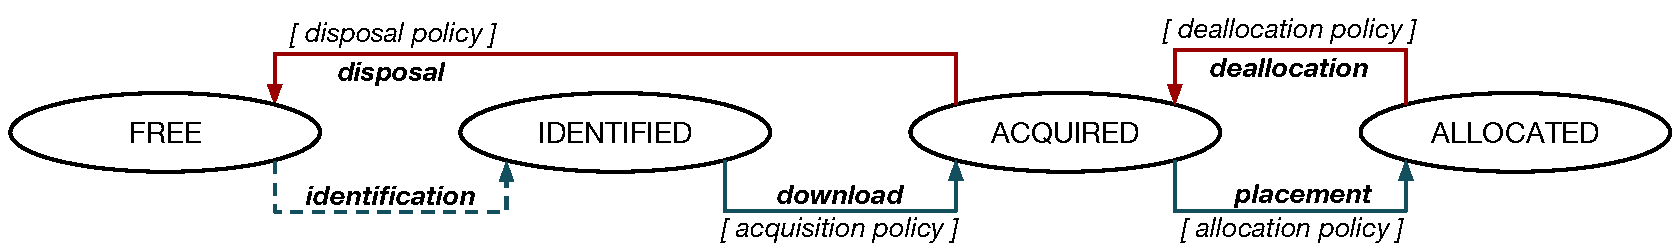
\includegraphics[width=0.95\textwidth]{figs/A3-E-domain}}\hfill
	
	\subfloat[Different states of a given client with respect to a given edge domain; the transitions between states triggered by client events are guarded by policies that may vary according to the client requirements\label{fig:A3-E-client}] {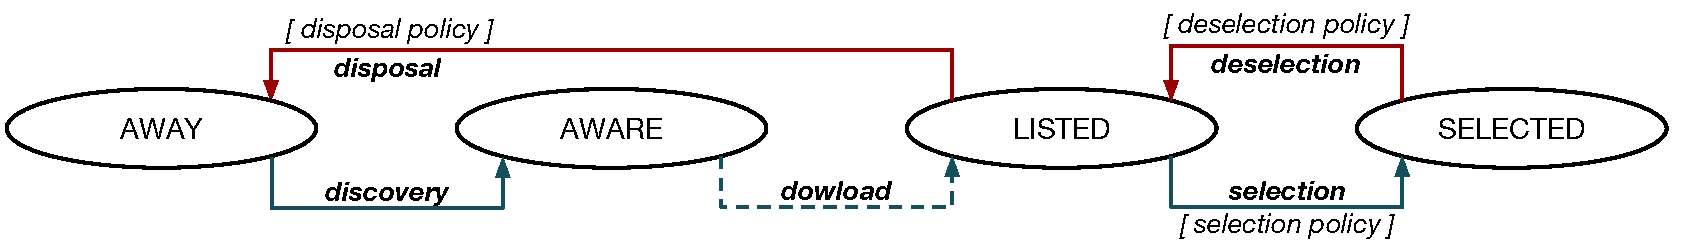
\includegraphics[width=0.95\textwidth]{figs/A3-E-client}}\hfill
	\caption{States and transitions among A3-E phases} \label{fig:A3-E-states}
\end{figure}


%What: the flexibility of A3-E model in terms of policies that regulate the transition among phases

The A3-E process is also flexible with respect to the transitions among subsequent phases. In particular, distinct policies may define different behaviors for the transition. Figures~\ref{fig:A3-E-domain} and~\ref{fig:A3-E-client} depict, respectively, the possible transitions among states of a domain with respect to a client application and vice-versa. Each state is mapped to the corresponding phase in Fig.~\ref{fig:A3-E-model}. 

From the domain perspective, policies affect the following conflicting properties: a) the \textit{efficiency} of domain resource usage; and b) the service setup \textit{delay}. Considering the first request arrival ($FRA$) from a client application as the reference event, the more \textit{reactive} the policies are to that event, the less time domain resources are likely to remain idle before it happens (more efficiency). In contrast, the chances of underutilization and idleness are higher with \textit{proactive} policies (less efficiency). Eq.~\ref{eq:setup_cost} models the total delay of service setup:

\begin{equation}\label{eq:setup_cost}
C_{SETUP} = C_{OFFLINE} + C_{RUNTIME}
\end{equation}

\noindent
in which the first term ($C_{OFFLINE}$) represents the resources required for downloading and installing the services (e.g., network and storage), whilst the later ($C_{RUNTIME}$) represents the resources needed for executing the services (e.g., memory and CPU). 

From the delay point of view, the relation is the opposite: the more \textit{reactive} the policies are with respect to the first request arrival event, the higher the delay the first request to each service is served with. In the other direction, the more \textit{pro-actively} services are made ready for execution, the lower the delay the first request to each of these services is served with. Eq.~\ref{eq:setup_delay} models the total delay of service setup:

%\Delta_{NET} + 
\begin{equation}\label{eq:setup_delay}
L_{SETUP} = \Delta_{AW} + \Delta_{AQ} + \Delta_{AL}
\end{equation}

\noindent
in which the first term ($\Delta_{AW}$) represents the time it takes for clients and domains to become aware of each other. The second term ($\Delta_{AQ}$) represents the time for acquiring all assets of a specific service, whilst the last term ($\Delta_{AL}$) represents the time for allocating resources for the service execution. 

For instance, existing cloud-based FaaS platforms (e.g., Amazon Lambda, Google Cloud Functions, and Apache OpenWhisk) employ on demand allocation of stateless functions, i.e., functions are reactively allocated upon arrival of the first request. Depending on the policy configuration, the platform waits for an idleness interval before deallocating the function~\footnote{\url{https://read.acloud.guru/how-long-does-aws-lambda-keep-your-idle-functions-around-before-a-cold-start-bf715d3b810}}. In these cases, the improved efficiency of the platform in allocating computational resources has the drawback of a setup delay (cold start). 

The domain-side policies in Fig.~\ref{fig:A3-E-domain} can be refined into three types: \textit{proactive} (P), \textit{sequential} (S), and \textit{reactive} (R). 

\begin{itemize}

\item \textbf{Proactive}: acquisition phase starts upon external event preceding the $FR_A$ event (e.g., the prediction of service usage in the near-future). Benefits: first response delay ($FR_D$) does not include $\Delta_{AQ}$. Drawback: acquired artifacts remain idle until usage. Example: stateless functions required by body device applications during a marathon event are fetched the night before the event by mobile-edge domains located along the course. 

\item \textbf{Sequential}: the beginning of acquisition phase is dictated by the completion of the awareness phase. Benefits: service artifacts are only acquired upon detection of a potential client in the domain coverage area, minimizing the likelihood of idleness. Drawbacks: $FR_D$ may include a fraction of $\Delta_{AQ}$ if $FRA$ precedes the end of acquisition. Example: stateless functions to be consumed by a mobile multiplayer game application are acquired by an indoor-edge domain inside a passenger train upon detection of two or more clients in the train.

\item \textbf{Reactive}: acquisition phase starts upon detection of a $FRA$. Benefits: acquisition of service artifacts follows an actual demand, eliminating artifacts storage idleness. Drawbacks: $FR_D$ includes $\Delta_{AQ}$, which may be disruptive for some applications. Example: stateless functions to be consumed by a TODO 

%the notion of a reactive allocation can be extended also to the acquisition of service artifacts. Instead of having functions pre-downloaded and installed, this process could happen in reaction to the first arrival of a request. 

\end{itemize}

In turn, the allocation phase can be triggered according to the following policies:

%The \textit{allocation policies} in Fig.~\ref{fig:A3-E-domain} can be:

\begin{itemize}

\item \textbf{Proactive}: allocation phase starts upon external event preceding the arrival of the first request (e.g., the prediction of service usage in the near-future). Benefits: $FR_D$ does not include $\Delta_{AL}$. Drawback: allocated resources remain idle until $FR_A$. Example: stateless functions to be consumed by connected vehicles are pre-allocated by mobile-edge domains in specific day times.

\item \textbf{Sequential}: allocation phase starts as soon as acquisition phase finishes. Benefits: depends on the acquisition policy. Drawbacks: depends on the acquisition policy. Example: stateless functions required by a marathon application running on body devices are allocated following their acquisition by the mobile-edge domains along the course.

\item \textbf{Reactive}: allocation phase starts as soon as $FR_A$ is detected. Benefits: eliminates idleness by conditioning allocation to an actual service demand. Drawback: $FR_D$ includes $\Delta_{AL}$ (cold start). Example: stateless functions required by a mobile multiplayer game are allocated by a local-edge domain inside a train following the detection of a $FR_A$ event.

\end{itemize}

%
%\begin{itemize}
%	
%	\item \textbf{Proactive}: . Benefits: . Drawback: . Example: .
%	
%	\item \textbf{Reactive}: . Benefits: . Drawback: . Example: .
%	
%\end{itemize}
%
%
%\begin{itemize}
%	
%	\item \textbf{Proactive}: . Benefits: . Drawback: . Example: .
%	
%	\item \textbf{Reactive}: . Benefits: . Drawback: . Example: .
%	
%\end{itemize}
%
%
%\subsubsection{Client-Side Policies}
%
%Clients may also adopt different policies for the selection and deselection of domains (Fig.~\ref{fig:A3-E-client}), namely:
%
%%domains are selected based on their category (cloud, edge, local) or/and 
%
%\begin{itemize}
%	
%	\item \textit{Selection policy}
%	
%	\begin{itemize}
%		
%		\item \textbf{Proactive}: 
%		
%		\item \textbf{Reactive}: 
%		
%	\end{itemize}
%	
%	\item \textit{Deselection policy}
%	
%	\begin{itemize}
%		
%		\item \textbf{Proactive}: 
%		
%		\item \textbf{Reactive}: 
%		
%	\end{itemize}
%\end{itemize}


%
%\subsection{Reference Architecture}
%
%\begin{figure}[tbp]
%	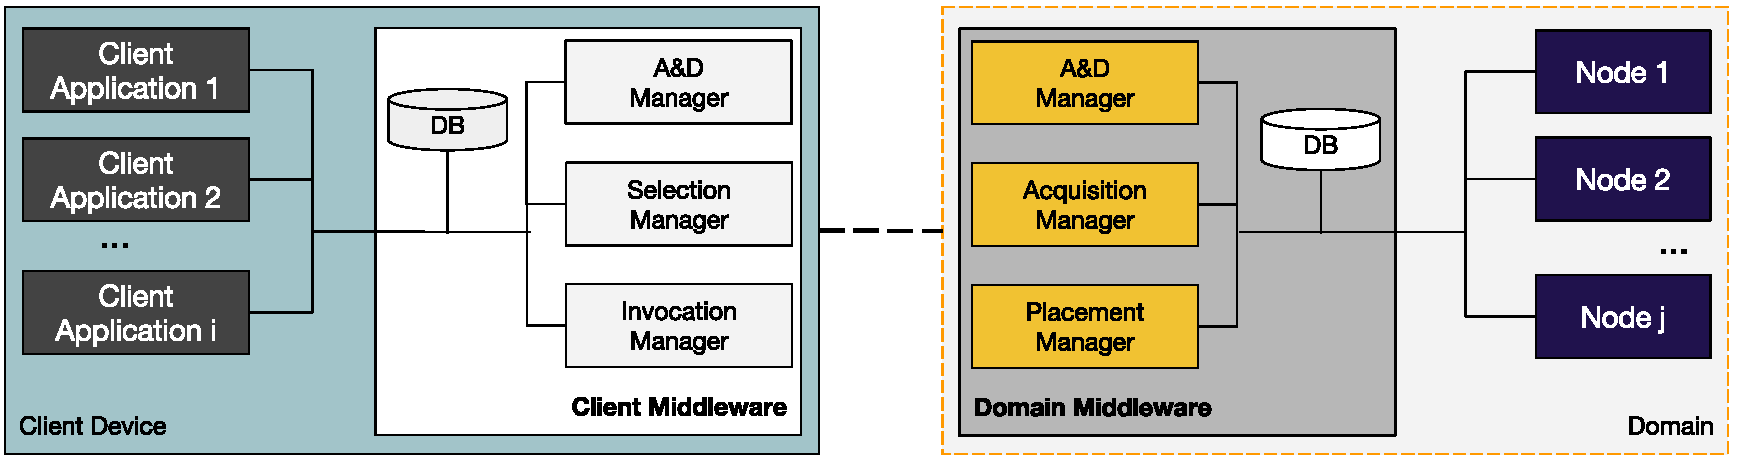
\includegraphics[width=.95\textwidth]{figs/A3-E-reference-architecture}
%	\caption{A3-E architecture in Mobile Devices and Edge Domains}
%	\label{fig:reference-architecture}
%	\end{figure}
	
